\documentclass[a4paper, 10pt]{article}
\usepackage[T1]{fontenc}
\usepackage[utf8]{inputenc}
\usepackage[slovene]{babel}
\usepackage{csquotes}
\usepackage{float}
\usepackage{lmodern}
\usepackage{amsmath}
\usepackage{leftidx}
%\usepackage[backend=biber, style=numeric]{biblatex}
\usepackage{amssymb}
\usepackage{amsthm}
\usepackage{amsfonts}
\usepackage{enumerate}
\usepackage{graphicx}
\usepackage{wrapfig}
\usepackage{amsthm}
\usepackage{mathrsfs}
\usepackage{mathtools}
\usepackage{url}
\usepackage{subfigure}
\usepackage{multirow}
\usepackage{lipsum}
\usepackage{wrapfig}
\usepackage{tikz}
\usepackage[format=plain, font=small, labelfont=bf, textfont=it, justification=centerlast]{caption}
\usepackage{booktabs}
\usepackage{siunitx}

\newtheorem{izr}{Izrek}
\newtheorem{posl}{Posledica}[izr]

\newcounter{defcount}
\newcounter{opombe}
\newcounter{vprcount}

\newenvironment{opomba}{\begin{flushleft}\stepcounter{opombe}\textbf{Opomba \arabic{opombe}:}}{\hfill\end{flushleft}}
\setlength{\parindent}{0mm}

\newenvironment{Vpr}{\begin{flushleft}\stepcounter{vprcount}\textbf{Vprašanje \arabic{vprcount}:}}{\hfill\end{flushleft}}
\setlength{\parindent}{0mm}

\newenvironment{Rešitev}{\begin{flushleft}\textit{Rešitev:}}{\hfill\end{flushleft}}
\setlength{\parindent}{0mm}

\newenvironment{definicija}{\begin{flushleft}\stepcounter{defcount}\textbf{Definicija \arabic{defcount}:}}{\hfill\end{flushleft}}
\setlength{\parindent}{0mm}

\newcommand{\naslov}[1]{\textit{#1}}
\newcommand{\abs}[1]{\ensuremath{\lvert #1 \rvert}}
\newcommand{\mth}[1]{\ensuremath{\mathbb{#1}}}
\newcommand{\R}{\mth{R}}
\newcommand{\Z}{\mth{Z}}
\newcommand{\Zp}{\mth{Z}^{+}}
\newcommand{\N}{\mth{N}}
\newcommand{\No}{\mth{N}_0}
\newcommand{\C}{\mth{C}}
\newcommand{\Q}{\mth{Q}}
\newcommand{\Qu}{\mth{Q}_u}
\newcommand{\pojem}[1]{\emph{#1}}
\newcommand{\con}{\ensuremath{\mathscr{C}}}
\newcommand{\padex}[2]{\ensuremath{{#1}^{\underline{#2}}}}
\newcommand{\rastx}[2]{\ensuremath{{#1}^{\bar{#2}}}}
\newcommand{\map}[3]{\ensuremath{{#1}: {#2} \rightarrow {#3}}}
\newcommand{\pra}[3]{{#1}{\ast}({#2}) = {#3}}

\title{Projektna naloga pri predmetu Numerična analiza in izbrana poglavja iz dinamičnih sistemov}
\date{21.~5.~2025}
\author{Jimmy Zakeršnik}
%===============================================================================
\begin{document}
	\maketitle
	\thispagestyle{empty}
	\newpage
	\section{Uvod}
		Ta naloga je razdeljena na dva dela. V prvem delu obravnavamo razna vprašanja v povezavi s podanimi polinomi $f_1, f_2, f_3, f_4$ in $f$ v spremenljivkah $x_1, x_2, x_3$ in $x_4$ s pomočjo programa Singular. Vsa koda, ki smo jo pri tem uporabili, je zbrana v datoteki ">\emph{polinomi 1.txt}"<, izpis programa pa je shranjen v datoteki ">\emph{VseVEnem.txt}"<. V drugem delu obravnavamo mehaniko amortizerja preko pripadajoče navadne diferencialne enačbe $2.$ reda s pomočjo programa MATLAB. Vsa koda, ki smo jo pri tem uporabili, je zbrana v datoteki ">\emph{amortizer2.m}"<.
%%%%%%%%%%%%%%%%%%%%%%%%%%%%%%%%%%%%%%%%%%%%%%%%%%%%%%%%%%%%%%%%%%%%%%%%%%%%%%%%
	\section{Prvi del}
		Na začetku določimo konstanti $A$ in $B$ v predpisu polinomov. V tem primeru je $A = 11$ in $B=24$, v skladu z danimi navodili. Tukaj omenimo še, da kadar naloga eksplicitno ne poda polja, v katerem rešujemo problem, kot privzeto vzamemo polje racionalnih števil in kot privzeto urejenost polinomov vzamemo leksikografsko ureditev. Definirajmo sedaj še polinomski ideal $I = <f_1, f_2, f_3, f_4 >$.
%%%%%%%%%%%%%%%%%%%%%%%%%%%%%%%%%%%%%%%%%%%%%%%%%%%%%%%%%%%%%%%%%%%%%%%%%%%%%%%%
		\begin{Vpr}
			Izračunajte Gröbnerjevo bazo ideala $I$ glede na \emph{lex}, \emph{deglex} in \emph{degrevlex} urejenost. Ali so pridobljene baze iste? Kateri izračun je bil najhitrejši?
		\end{Vpr}
%%%%%%%%%%%%%%%%%%%%%%%%%%%%%%%%%%%%%%%%%%%%%%%%%%%%%%%%%%%%%%%%%%%%%%%%%%%%%%%%		
		\begin{Rešitev}
		 	Vsaka izračunana baza je prostorsko obsežna in zato ne bo eksplicitno podana v tej datoteki. Poračunane baze se izpišejo ob zagonu datoteke ">\emph{polinomi 1.txt}"<, so pa shranjene tudi v datoteki ">\emph{VseVEnem.txt}"<. Kljub temu je enostavno priti do odgovorov na zastavljeno vprašanje: Pridobljene Gröbnerjeve baze so različne, čas izračuna pa je (z uporabo funkcije \emph{groebner}) v vseh primerih enak.
		\end{Rešitev}
%%%%%%%%%%%%%%%%%%%%%%%%%%%%%%%%%%%%%%%%%%%%%%%%%%%%%%%%%%%%%%%%%%%%%%%%%%%%%%%% 
		\begin{Vpr}
		 	Izračunajte dekompozicijo raznoterosti ideala $I$ nad poljem racionalnih števil. Koliko komponent vsebuje dekompozicija raznoterosti ideala $I$ nad poljem realnih števil? Kaj pa nad poljem kompleksnih števil?
		\end{Vpr}
%%%%%%%%%%%%%%%%%%%%%%%%%%%%%%%%%%%%%%%%%%%%%%%%%%%%%%%%%%%%%%%%%%%%%%%%%%%%%%%%
		\begin{Rešitev}
		 	V tej nalogi smo najprej poračunali dekompozicijo ideala $I$ nad poljem racionalnih števil, z uporabo funkcije \emph{minAssGTZ}. Hitro opazimo, da ima pripadajoča raznoterost v tem primeru tri (ireducibilne) komponente. Od teh je prva komponenta $0$-razsežna: $$(x1, x2, x3, x4) = (-11.546501, 389.6288, -167.98446, -0.17786659).$$ Ko se premaknemo v polje realnih števil, se število komponent ne spremeni, saj so vse preostale ničle sistema, ki ga določa $0$-razsežna komponenta dekompozocije, kompleksne, in tudi v nobeni drugi komponenti ne pridobimo nobene nove rešitve. Nad poljem kompleksnih števil, število ireducibilnih komponent dekompozicije naraste na $11$, saj sedaj lahko dodamo vse kompleksne ničle sistema, ki določa prvo komponento. Premik v polje kompleksnih števil tudi poveča razsežnost tretje komponente, ki je določena z enačbo $$x_1^2 + 1225x_2^2 = 0,$$ a s tem ne poveča števila komponent dekompozicije.
		\end{Rešitev}
%%%%%%%%%%%%%%%%%%%%%%%%%%%%%%%%%%%%%%%%%%%%%%%%%%%%%%%%%%%%%%%%%%%%%%%%%%%%%%%%
		\begin{Vpr}
		 	Izračunajte primarno dekompozicijo raznoterosti ideala $I$.
		\end{Vpr}
%%%%%%%%%%%%%%%%%%%%%%%%%%%%%%%%%%%%%%%%%%%%%%%%%%%%%%%%%%%%%%%%%%%%%%%%%%%%%%%%
		\begin{Rešitev}
			Primarna dekompozicija je bila izračunana z ukazom \emph{primdec} in je v celoti izpisana v datoteki ">\emph{VseVEnem.txt}"<.
		\end{Rešitev}
%%%%%%%%%%%%%%%%%%%%%%%%%%%%%%%%%%%%%%%%%%%%%%%%%%%%%%%%%%%%%%%%%%%%%%%%%%%%%%%%
		\begin{Vpr}
			Če je komponenta dekompozicije raznoterosti ideala $I$ $0$-dimenzionalna, navedite točke komponente (numerično). V nasprotnem primeru navedite parametrizacijo komponente nad poljem realnih števil.
		\end{Vpr}
%%%%%%%%%%%%%%%%%%%%%%%%%%%%%%%%%%%%%%%%%%%%%%%%%%%%%%%%%%%%%%%%%%%%%%%%%%%%%%%%
		\begin{Rešitev}
			Točka, ki sestavlja $0$-razsežne komponente dekompozicije nad poljem realnih števil, je predstavljena v datoteki ">\emph{VseVEnem.txt}"<. Nad tem istim poljem, ima komponenta, ki jo določa enačba $$24x_3 + 11 = 0,$$ parametrizacijo $$(x_1, x_2, x_4)\mapsto(x_1, x_2, -\frac{11}{24}, x_4),$$ komponenta, določena z enačbo $$x_1^2 + 1225x_2^2 = 0,$$ pa $$(x_3, x_4) \mapsto (0, 0, x_3, x_4).$$
		\end{Rešitev}
%%%%%%%%%%%%%%%%%%%%%%%%%%%%%%%%%%%%%%%%%%%%%%%%%%%%%%%%%%%%%%%%%%%%%%%%%%%%%%%%
		\begin{Vpr}
			Ali je polinom $f$ v idealu $I$?
		\end{Vpr}
%%%%%%%%%%%%%%%%%%%%%%%%%%%%%%%%%%%%%%%%%%%%%%%%%%%%%%%%%%%%%%%%%%%%%%%%%%%%%%%%
		\begin{Rešitev}
			Z uporabo ukaza \emph{reduce} vidimo, da polinom $f$ ni element ideala $I$.
		\end{Rešitev}
%%%%%%%%%%%%%%%%%%%%%%%%%%%%%%%%%%%%%%%%%%%%%%%%%%%%%%%%%%%%%%%%%%%%%%%%%%%%%%%%
		\begin{Vpr}
			Izračunajte $I : <x_1^2 + (A + B)^2x_2^2 >$. Razložite geometrijski pomen rezultata.
		\end{Vpr}
%%%%%%%%%%%%%%%%%%%%%%%%%%%%%%%%%%%%%%%%%%%%%%%%%%%%%%%%%%%%%%%%%%%%%%%%%%%%%%%%
		\begin{Rešitev}
			Kvocientni ideal je v celoti zapisan v datoteki ">\emph{VseVEnem.txt}"<. Ko s pomočjo ukaza \emph{minAssGTZ} poračunamo dekompozicijo raznoterosti danega kvocientnega ideala opazimo, da se je število komponent, glede na ideal $I$, zmanjšalo! Bolj natančno, ">izgubila"< se je komponenta, določena z enačbo $$x_1^2 + 1225x_2^2 = 0.$$
		\end{Rešitev}
%%%%%%%%%%%%%%%%%%%%%%%%%%%%%%%%%%%%%%%%%%%%%%%%%%%%%%%%%%%%%%%%%%%%%%%%%%%%%%%%
		\begin{Vpr}
			Naj bosta $H = <f, f_4>$ in $J = <f_1, f_2, f_3>$. Ali sta ideala $H$ in $J$ enaka?
		\end{Vpr}
%%%%%%%%%%%%%%%%%%%%%%%%%%%%%%%%%%%%%%%%%%%%%%%%%%%%%%%%%%%%%%%%%%%%%%%%%%%%%%%%
		\begin{Rešitev}
			To nalogo smo rešili tako, da smo najprej poračunali Gröbnerjevi bazi obeh idealov ter nato preverili, ali lahko vsak element baze enega ideala reduciramo z bazo drugega. To se seveda ne da storiti, torej sta ideala $H$ in $J$ različna.
		\end{Rešitev}
%%%%%%%%%%%%%%%%%%%%%%%%%%%%%%%%%%%%%%%%%%%%%%%%%%%%%%%%%%%%%%%%%%%%%%%%%%%%%%%%
		\begin{Vpr}
			Izračunajte $H + J$ in presek idealov $H$ in $J$. Razložite geometrijski pomen rezultatov.
		\end{Vpr}
%%%%%%%%%%%%%%%%%%%%%%%%%%%%%%%%%%%%%%%%%%%%%%%%%%%%%%%%%%%%%%%%%%%%%%%%%%%%%%%%
		\begin{Rešitev}
			Tako vsota kot presek idealov sta zapisana v datoteki ">\emph{VseVEnem.txt}"<. Izkaže se, da je raznoterost, ki jo določa vsota danih idealov, sestavljena iz dveh komponent. Enostavno je videti, da je rna izmed teh komponent podmnožica ene izmed komponent ideala $I$. To seveda ni presenetljivo, saj ideal $H + J = <f_1, f_2, f_3, f_4, f>$ vsebuje ideal $I$. Zato lahko sklepamo celo, da je celotna raznoterost ideala $H+J$ vsebovana v raznoterosti ideala $I$. Po drugi strani, razcep raznoterosti ideala $H\cap J$ pokaže, da ta ideal v celoti vsebuje več-razsežni komponenti razcepa ideala $I$, ter še dve dodatni komponenti. Če v prvi polinom prve komponente in prvi polinom druge komponente vstavimo točko $0$-razsežne komponente ideala $I$, torej $$(x_1, x_2, x_3, x_4)=(-11.546501, 389.6288, -167.98446, -0.17786659),$$ pa opazimo, da ta točka ni vsebovana v nobeni od omenjenih komponent. Res, ko vstavimo to točko v polinom $5x_2^2+290x_2+48x_3^2+2976x_3x_4$, dobimo približen rezultat $2315466,121$, ko jo vstavimo v polinom \begin{align*}
				20736x_3^3&+2553435x_3^2+27441792x_3x_4-138171264x_3 +\\ &+84652032x_4^2-841420800x_4+2057487872,
			\end{align*} pa je rezultat približno $-1503,215$. To pomeni, da raznoterost ideala $I$ ni vsebovana v raznoterosti ideala $H\cap J$, ima pa z njo neprazen presek.
		\end{Rešitev}
%%%%%%%%%%%%%%%%%%%%%%%%%%%%%%%%%%%%%%%%%%%%%%%%%%%%%%%%%%%%%%%%%%%%%%%%%%%%%%%%
	\section{Drugi del}
	\setcounter{vprcount}{0}
		Podan imamo amortizer v katerem s $K$ označimo koeficient vzmeti, s $\alpha$ viskoznost tekočine ter z $m$ maso avtomobila. Z $x(t)$ označimo oddaljenost dna avtomobila od začetne mirovne lege. Ko upoštevamo Newtonov $2.$ zakon, dobimo enačbo $$m\overset{..}{x} = -\alpha\dot{x} - Kx,$$ oziroma $$\overset{..}{x} +\frac{\alpha}{m}\dot{x} + \frac{K}{m}x = 0.$$ Sedaj vpeljemo oznaki $2k = \frac{\alpha}{m}$ in $\omega^2 = \frac{K}{m}$ ter tako dobimo končno obliko enačbe amortizerja: \begin{equation}
			\label{eq:amort}
		\overset{..}{x} +2k\dot{x} + \omega^2x = 0.
		\end{equation}
%%%%%%%%%%%%%%%%%%%%%%%%%%%%%%%%%%%%%%%%%%%%%%%%%%%%%%%%%%%%%%%%%%%%%%%%%%%%%%%%
		\begin{Vpr}
			Zapiši enačbo \ref{eq:amort} v ekvivalentni obliki kot dvorazsežni linearni sistem diferencialnih enačb.
		\end{Vpr}
%%%%%%%%%%%%%%%%%%%%%%%%%%%%%%%%%%%%%%%%%%%%%%%%%%%%%%%%%%%%%%%%%%%%%%%%%%%%%%%%
		\begin{Rešitev}
			Da enačbo \ref{eq:amort} prepišemo v ekvivalentno obliko kot dvorazsežni linarni sistem diferencialnih enačb, uvedemo novo spremenljivko $y = \dot{x}$. Ko to vstavimo v enačbo \ref{eq:amort}, dobimo enačbo $$\dot{y} + 2ky + \omega^2x = 0.$$ Sedaj izpostavimo $\dot{y}$ in tako dobimo iskani sistem: \begin{equation}
				\label{eq:amort2}
				\begin{bmatrix}
					\dot{x} \\
					\dot{y}
				\end{bmatrix}=  \begin{bmatrix}
				y\\ -\omega^2x - 2ky
				\end{bmatrix}
			\end{equation}
		\end{Rešitev}
%%%%%%%%%%%%%%%%%%%%%%%%%%%%%%%%%%%%%%%%%%%%%%%%%%%%%%%%%%%%%%%%%%%%%%%%%%%%%%%%
		\begin{Vpr}
			Izberi parametra $k>0$ in $\omega>0$ tako, da ima matrika sistema: \begin{enumerate}[a)]
				\item dve realni lastni vrednosti,
				\item eno realno lastno vrednost,
				\item dve kompleksni lastni vrednosti.
			\end{enumerate}
		\end{Vpr}
%%%%%%%%%%%%%%%%%%%%%%%%%%%%%%%%%%%%%%%%%%%%%%%%%%%%%%%%%%%%%%%%%%%%%%%%%%%%%%%%
		\begin{Rešitev}
				Sistemu \ref{eq:amort2} pripada matrika $A = \begin{bmatrix}
				0 & 1 \\
				-\omega^2 & -2k
			\end{bmatrix}$. Pripadajoči karakteristični polinom se glasi: $$p(\lambda) = det(A - \lambda I) = (-\lambda)(-2k-\lambda) + \omega^2 = \lambda^2 + 2k\lambda + \omega^2 .$$ Ničli tega polinoma, torej lastni vrednosti matrike $A$, bosta ravno $$ \lambda_{1, 2} = \frac{-2k \pm \sqrt{4k^2 - 4\omega^2}}{2} = -k \pm \sqrt{k^2 - \omega^2}.$$ Sedaj določimo parametra $k>0$ in $\omega >0$ tako, da bodo lastne vrednosti zadoščale pogojem:
			\begin{enumerate}[a)]
				\item Da bi obe lastni vrednosti bili različni in realni, mora biti izraz pod korenom, torej $k^2 - \omega^2$, pozitiven. Glede na to, da sta tako $k$ kot $\omega$ pozitivna parametra, to pomeni, da je potreben pogoj ravno, da je $k>\omega$. Če označimo $a^2 = k^2 - \omega^2$, sta potem lastni vrednosti pripadajočega sistema ravno $\lambda_1 = -k + a$ in $\lambda_2 = -k-a$.
				\item Da bi obe lastni vrednosti bili enaki in realni, mora biti izraz pod korenom, torej $k^2 - \omega^2$, enak $0$. To bo res natanko tedaj, ko bo $k^2 = \omega^2$ oziroma $k = \omega$ (saj sta $k$ in $\omega$ pozitivna). Posledično, je naša dvojna realna lastna vrednost ravno $\lambda_0 = -k$.
				\item Da bi obe lastni vrednosti bili različni in kompleksni, mora biti izraz pod korenom, torej $k^2 - \omega^2$, negativen. Upoštevajoč pogoja pozitivnosti parametrov $k$ in $\omega$ hitro vidimo, da je to ekvivalentno pogoju $k < \omega$. Če označimo $-b^2=k^2 - \omega^2$, sta potem pripadajoči kompleksni lastni vrednosti ravno $\lambda_1 = -k + ib$ in $\lambda_2=-k-ib$.
			\end{enumerate}
		\end{Rešitev}
%%%%%%%%%%%%%%%%%%%%%%%%%%%%%%%%%%%%%%%%%%%%%%%%%%%%%%%%%%%%%%%%%%%%%%%%%%%%%%%%
		\begin{Vpr}
			Za vsakega od primerov $a), b)$ in $c)$ iz prejšnje naloge nariši: \begin{enumerate}
				\item rešitev $x(t)$ v ravnini $(x, t)$.
				\item fazno sliko v ravnini $(x, \dot{x})$.
			\end{enumerate}
		\end{Vpr}
%%%%%%%%%%%%%%%%%%%%%%%%%%%%%%%%%%%%%%%%%%%%%%%%%%%%%%%%%%%%%%%%%%%%%%%%%%%%%%%%
		\begin{Rešitev}
			S pomočjo programa MATLAB narišemo graf rešitev in fazni portret za vse tri primere iz prejšnje naloge. Na vsakem grafu bo narisan šop rešitev v odvisnosti od začetnega pogoja. V tem primeru so začetni pogoji vsi elementi mreže $\{-3, -2, -1, 0, 1, 2, 3\}\times\{-3, -2, -1, 0, 1, 2, 3\}$.
			\begin{figure}[H]
				\centering
				\includegraphics[scale=0.5]{Rešitev1.png}
				\caption{Graf rešitve $x(t)$ v primeru dveh realnih lastnih vrednosti ($k=2, \omega=1$).}
							
				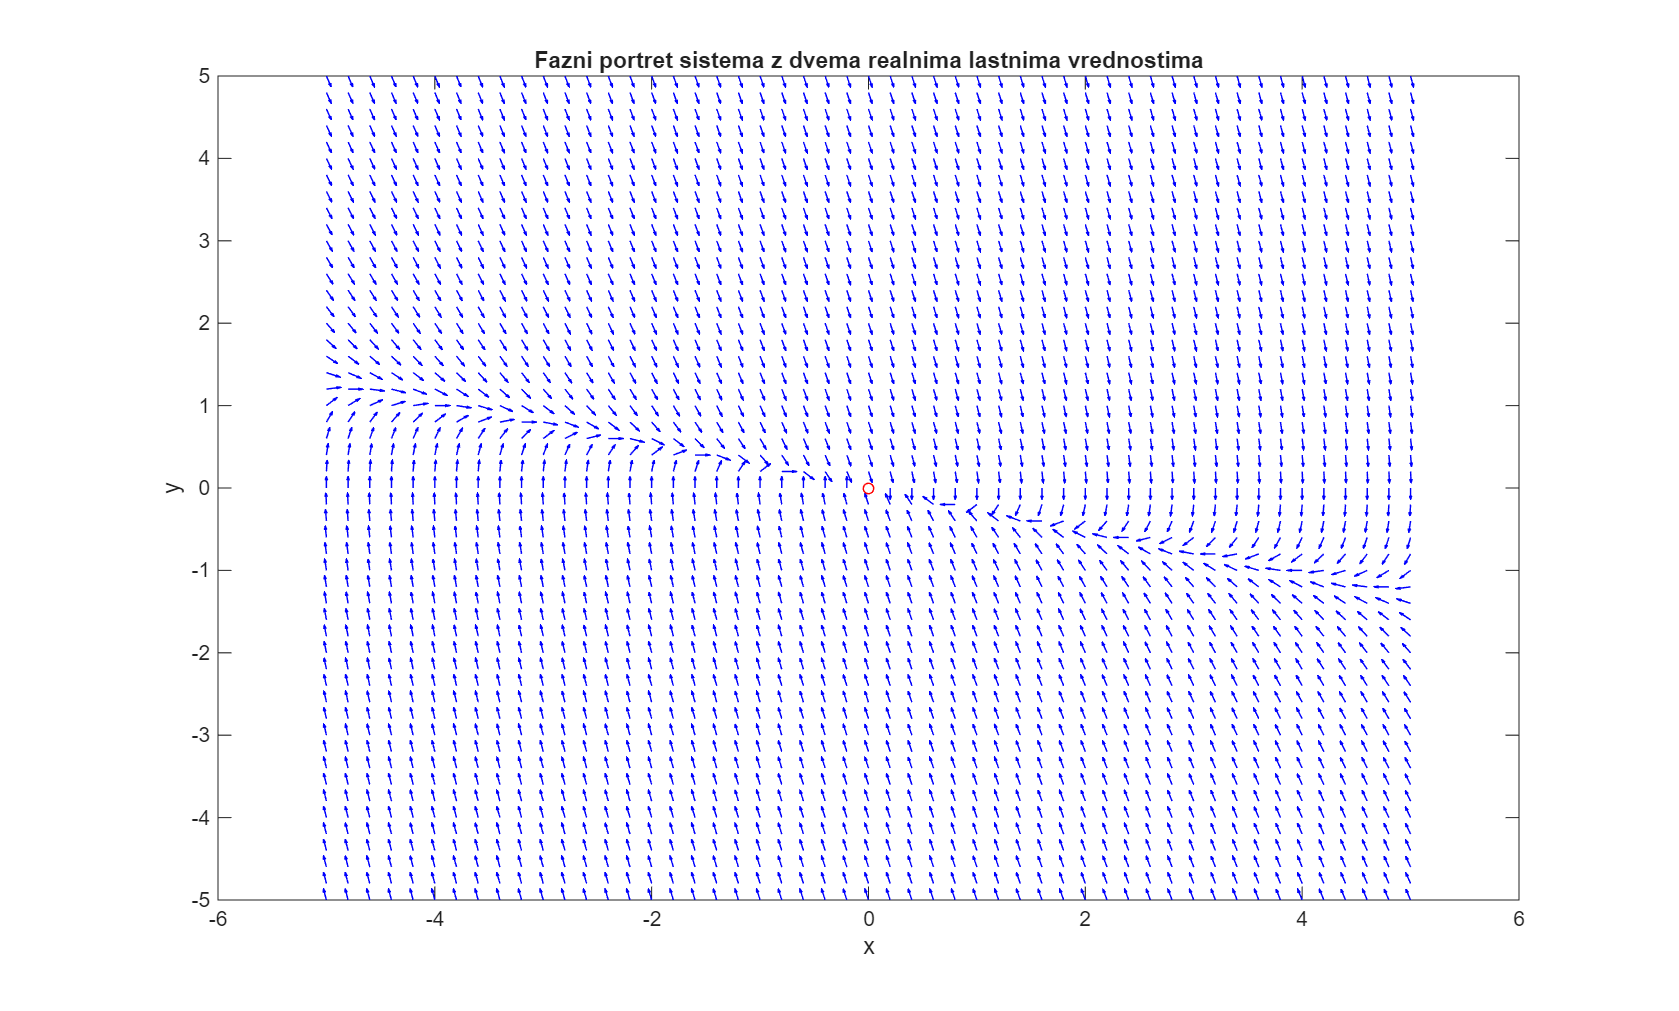
\includegraphics[scale=0.5]{Fazni1.png}
				\caption{Fazni portret sistema v primeru dveh realnih lastnih vrednosti ($k=2, \omega=1$).}
			\end{figure}
			
			%\pagebreak
			
			\begin{figure}[H]
				\includegraphics[scale=0.5]{Rešitev2.png}
				\caption{Graf rešitve $x(t)$ v primeru ene realne lastne vrednosti ($k=2, \omega=2$).}
			
				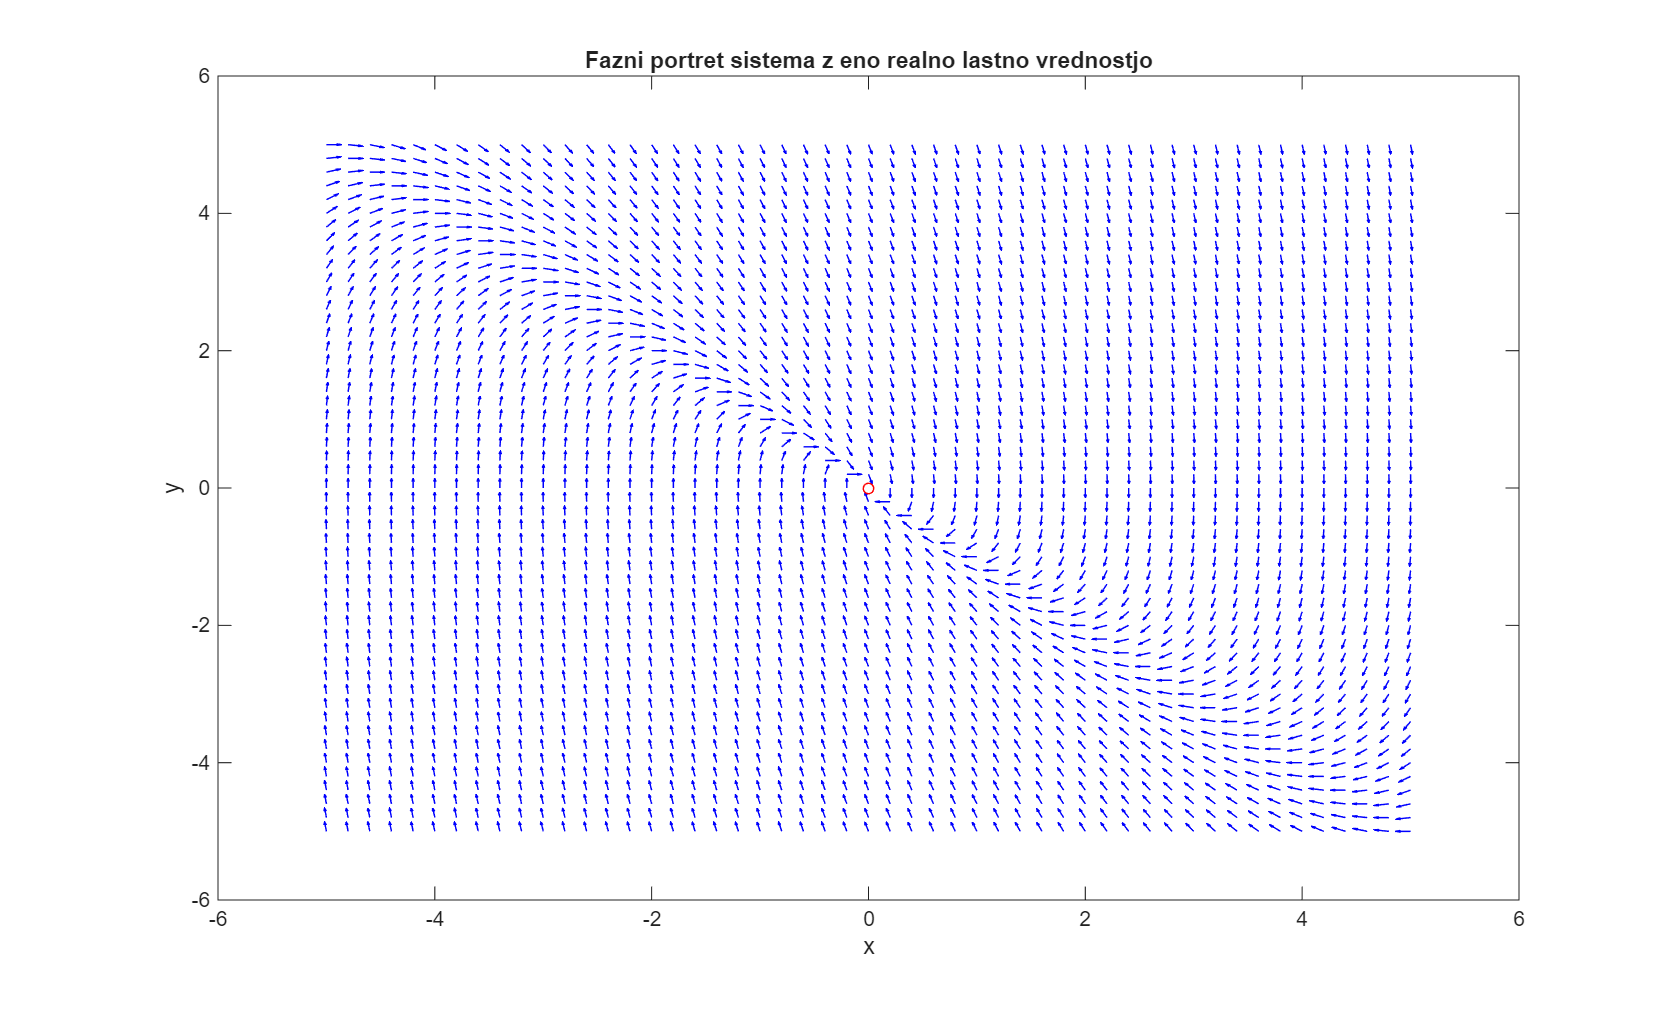
\includegraphics[scale=0.5]{Fazni2.png}
				\caption{Fazni portret sistema v primeru ene realne lastne vrednosti ($k=2, \omega=2$).}
			\end{figure}
			
			%\pagebreak
				
			\begin{figure}[H]
				\includegraphics[scale=0.5]{Rešitev3.png}
				\caption{Graf rešitve $x(t)$ v primeru dveh kompleksnih lastnih vrednosti ($k=1, \omega=2$).}
				
				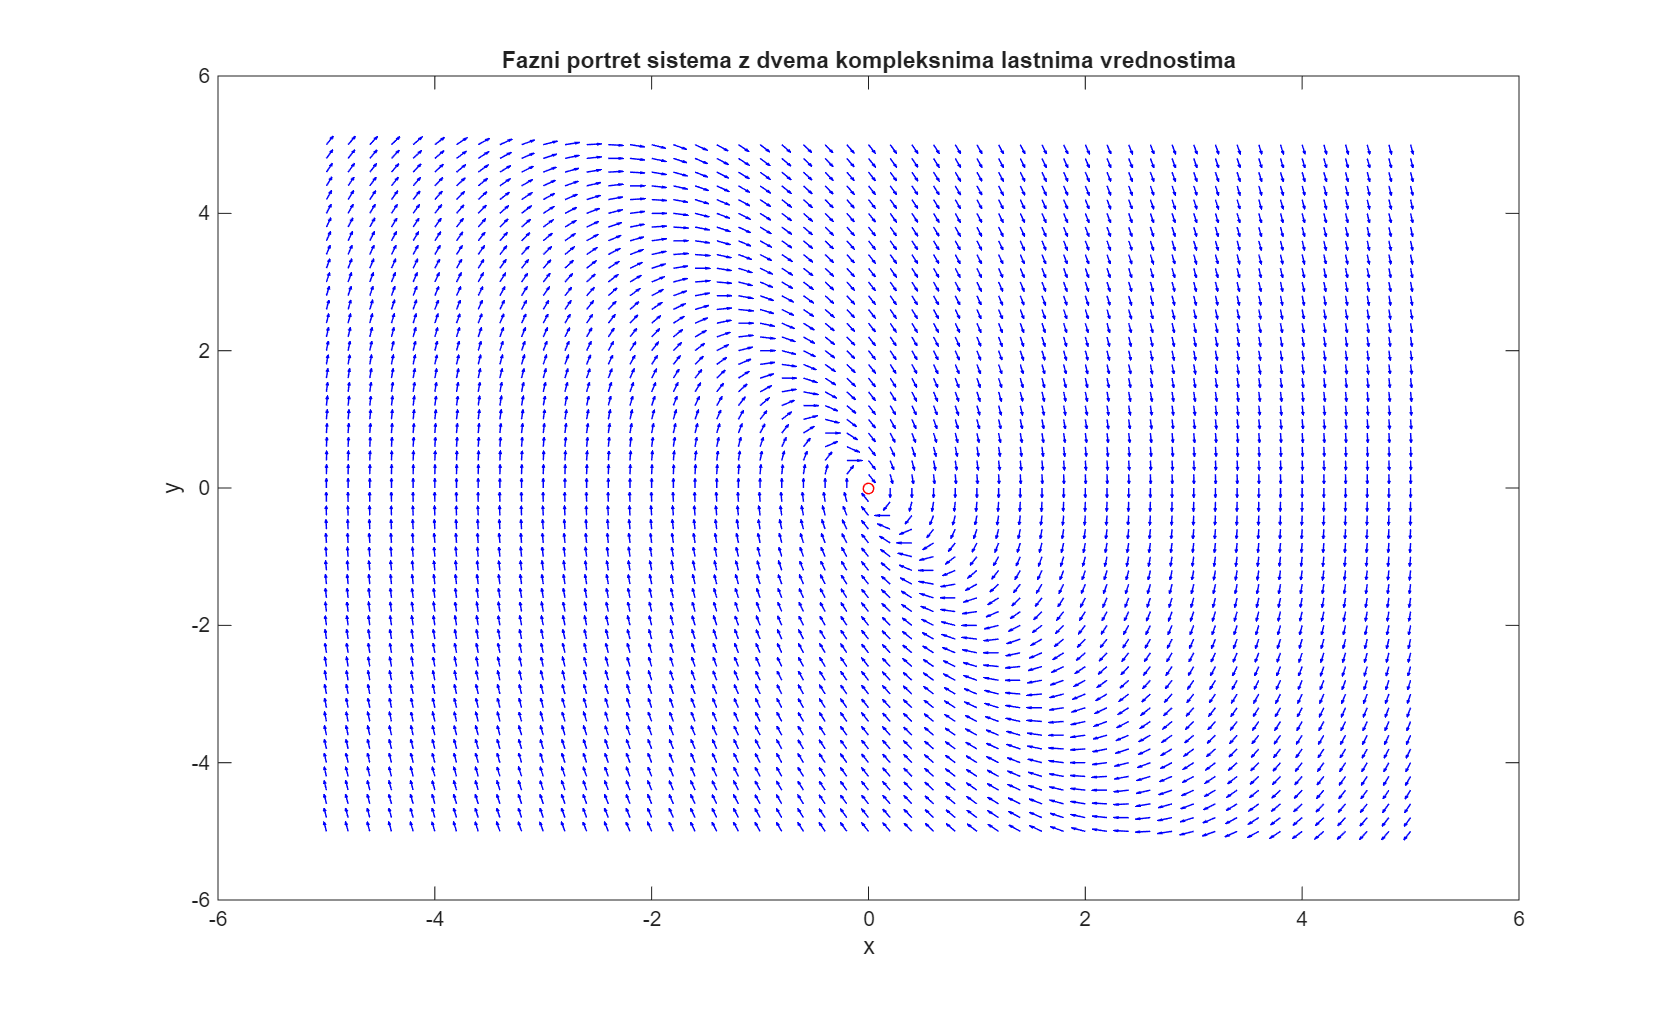
\includegraphics[scale=0.5]{Fazni3.png}
				\caption{Fazni portret sistema v primeru dveh kompleksnih lastnih vrednosti ($k=1, \omega=2$).}
			\end{figure}
		\end{Rešitev}
%%%%%%%%%%%%%%%%%%%%%%%%%%%%%%%%%%%%%%%%%%%%%%%%%%%%%%%%%%%%%%%%%%%%%%%%%%%%%%%%

		\begin{Vpr}
			Katera izbira parametrov je najbolj primerna za pravilno delovanje amortizerja?
		\end{Vpr}
%%%%%%%%%%%%%%%%%%%%%%%%%%%%%%%%%%%%%%%%%%%%%%%%%%%%%%%%%%%%%%%%%%%%%%%%%%%%%%%%
		\begin{Rešitev}
			Glede na fazni portret rešitve je najbolj primerna izbira parametrov $k$ in $\omega$, v kateri je $k<\omega$, torej tista, v kateri ima sistem dve kompleksni lastni vrednosti.
		\end{Rešitev}
%%%%%%%%%%%%%%%%%%%%%%%%%%%%%%%%%%%%%%%%%%%%%%%%%%%%%%%%%%%%%%%%%%%%%%%%%%%%%%%%
\end{document}